\chapter{Presentation of Kyushu University}
\section{Kyushu University}
\begin{figure}[htb!]
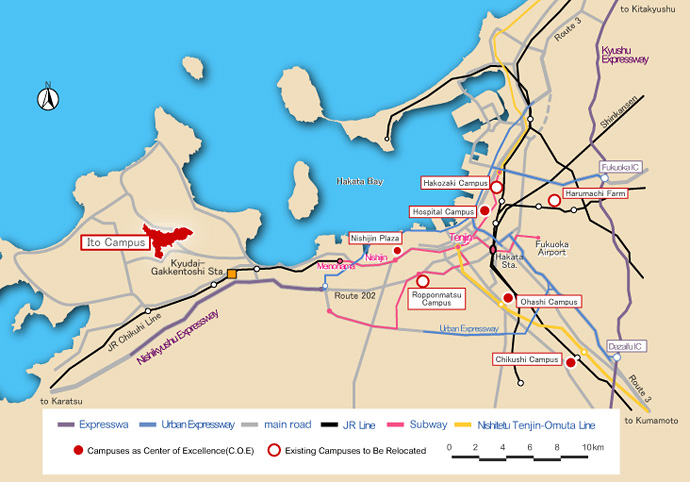
\includegraphics[width=\textwidth]{images/campusesMap.jpg}
\caption{Map of Kyushu University's campuses in Fukuoka. The $6^{th}$ campus is the Beppu campus, not included on this map. Map from \cite{greenAsia} .}
\label{fig:kyudaiCampuses}
\end{figure}

Kyushu University is a public university in Fukuoka, on the island of Kyushu in western Japan. iIt was founded in 1911 as the Kyushu Imperial University, and is currently the largest public university in Kyushu. It employs 2186 faculty members and has 18765 students, including more than 1700 international students \cite{kyushuWebsiteHistory}. Kyushu University is one of the best research universities in Japan according to Thomson Reuters, and especially shines in Materials Science, Chemistry, Biology and Biochemistry, Immunology as well as Pharmacology and Toxicology \cite{reutersResearchRanking}. It counts 12 undergraduate schools, 19 graduate schools, 16 graduate faculties and 8 research institutes \cite{kyushuWebsiteFaculties}, spread out on 6 campuses (\autoref{fig:kyudaiCampuses}).

\section{Faculty of design and the department of visual communication design}
\begin{figure}[htb!]
\includegraphics[width=\textwidth]{images/ohashi.jpg}
\caption{Ohashi Campus, home of the faculty of design. Photography courtesy of the author.}
\label{fig:ohashi}
\end{figure}
Kyushu University's faculty of design is located in Ohashi campus alongside the graduate school of design and the school of design. It includes various departments teaching and researching environmental design, visual communication design, art and information, industrial design, acoustic design, and others. The department of visual communication design includes the section of Image Engineering, which includes computer vision and machine learning \cite{facultyDesignWebsite}.

\section{Sakamoto laboratory}
The Sakamoto laboratory, part of the department of visual communication design, is supervised by eponymous teacher Hiroyasu Sakamoto. It specializes in computer vision, virtual reality and machine learning. It is constituted at the time of writing by 8 graduate students and 3 undergraduate students, including 4 foreign students. Domains currently researched in the laboratory include animation character image analysis, 3D mesh segmentation, face recognition and head-mounted devices (google glass like devices).
